\documentclass[10pt]{amsart}
\usepackage[left=.75in,right=.75in,top=.75in,bottom=.75in]{geometry}
\geometry{letterpaper}                   % ... or a4paper or a5paper or ... 
%\geometry{landscape}                % Activate for for rotated page geometry
%\usepackage[parfill]{parskip}    % Activate to begin paragraphs with an empty line rather than an indent
\usepackage{color,graphicx}
\usepackage{amssymb}
\usepackage{amsmath}
\usepackage{verbatim}
%\DeclareGraphicsRule{.tif}{png}{.png}{`convert #1 `dirname #1`/`basename #1 .tif`.png}
\newcommand{\eqn}[1]{(\ref{#1})}
\newcommand{\picdir}{./pdffig}

%\renewcommand{\labelenumi}{\arabic{enumi}. }

%http://latex2rtf.sourceforge.net/latex2rtf_1_9_19.html#Conditional-Parsing
%Starting with LaTeX2RTF 1.9.18, there is a handy method for
%controlling which content should be processed by LaTeX or by
%LaTeX2RTF . Control is achieved using the standard \if facility of
%TeX. If you include the following line in the preamble of your document 
%
%     \newif\iflatextortf
%Then you will create a new \iflatextortf command in LaTeX . TeX
%sets the value of this to false by default. Now, LaTeX2RTF
%internally sets \iflatextortf to be true, and to ensure that this
%is always the case, LaTeX2RTF ignores the command
%\latextortffalse. This means that you can control how different
%applications process your document by
%
%     \iflatextortf
%     This code is processed only by latex2rtf
%     \else
%     This code is processed only by latex
%     \fi
%Note that \iflatextortf will only work within a section; you
%cannot use this command to conditionally parse code that crosses
%section boundaries. Also, it will only work on complete table or
%figure environments. Due to the mechanism used by LaTeX2RTF in
%processing these environments, at this time the only way to
%conditionally parse tables and figures is to include two complete
%versions of the environment in question, nested within an
%appropriate \iflatextortf structure.
%
\newif\iflatextortf

\iflatextortf 
%do nothing
\else  %pdflatex
\usepackage{boxedminipage,float}
\usepackage{wrapfig,setspace}
\usepackage[pdftex, plainpages=false, colorlinks=true, citecolor=black, filecolor=black, linkcolor=black, urlcolor=black]{hyperref}

%% textureanat_ATROPOS_GMM.png                               
%% textureanat_ATROPOS_GMM_VOLUME_TO_SURFACE_AREA_RATIO.png  
%% textureanat_DENOISE.png                                   
%% textureanat_ATROPOS_GMM_CANNY.png
%% textureanat_ClusterProminence_1.png                 textureanat_ClusterProminence_5.png                     
%% textureanat_Energy_1.png                            textureanat_Energy_5.png                     
%% textureanat_Inertia_1.png                           textureanat_Inertia_5.png                    
%% textureanat_ClusterShade_1.png                      textureanat_ClusterShade_5.png               
%% textureanat_Entropy_1.png                           textureanat_Entropy_5.png                    
%% textureanat_InverseDifferenceMoment_1.png           textureanat_InverseDifferenceMoment_5.png    
%% textureanat_Correlation_1.png                       textureanat_Correlation_5.png                
%% textureanat_HaralickCorrelation_1.png               textureanat_HaralickCorrelation_5.png        



%% 
%%                
%%             
%% 
%%                
%%                
%%                

\title{Image Feature Data Service}

\author{
        D.~Fuentes\textsuperscript{1} 
}

\date{ \small
The University of Texas M.D. Anderson Cancer Center,\\
Departments of \textsuperscript{1}Imaging Physics, \textsuperscript{2}Diagnostic Radiology,
%\textsuperscript{3}Gastrointenstinal Oncology,
%and \textsuperscript{4}Biostatistics, 
Houston TX 77030, USA \\
%Email: \texttt{jhazle@mdanderson.org}   \\
Received: date / Accepted: date
% Webpage: \texttt{http://wiki.ices.utexas.edu/dddas}
}



\begin{document}
\maketitle

\begin{itemize}
  \item Hypothesis: Volumetric RECIST\cite{tacher2015comparison} provides
more reliable response to therapy than RECIST 1.x \begin{itemize}
      \item 'more reliable' = earlier response ?
      \item 'more reliable' = more accurate ?  
      \item How do we quantify this ?
    \end{itemize}
\end{itemize}

\begin{figure}[h]
  \IfFileExists{workdir/StatSummary.pdf}{\includegraphics[width=.8\textwidth]{workdir/StatSummary.pdf}  }{\fbox{\begin{picture}(10,10)\put(0,5){ not found } \end{picture}}}
  \IfFileExists{workdir/TopPredictors.csv}{\verbatiminput{workdir/TopPredictors.csv}}{predictors not found}
   \caption{Group Summary}\label{fig:GroupSummary}
\end{figure}
        
\begin{thebibliography}{1}

\bibitem{tacher2015comparison}
Vania Tacher, MingDe Lin, Rafael Duran, Hooman Yarmohammadi, Howard Lee,
Julius
  Chapiro, Michael Chao, Zhijun Wang, Constantine Frangakis, Jae~Ho Sohn,
  et~al.
\newblock Comparison of existing response criteria in patients with
  hepatocellular carcinoma treated with transarterial chemoembolization
using a
  3d quantitative approach.
\newblock {\em Radiology}, 278(1):275--284, 2015.

\end{thebibliography}

\pagebreak
\section{Usage}
\begin{figure}[h]
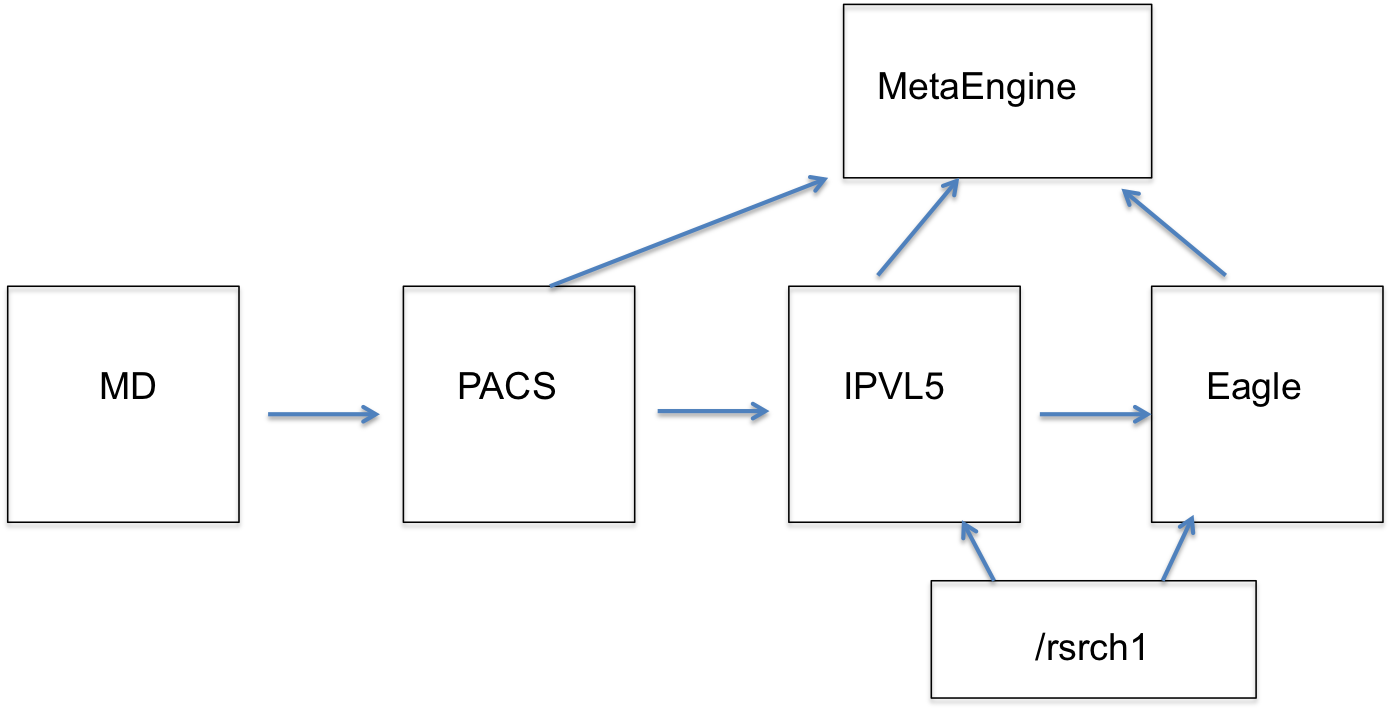
\includegraphics[width=1\textwidth]{\picdir/DataFlow.png}
\caption{
Data Service Workflow.
Medically trained user transfers studies from PACS to image 
processing dicom server for manual labeling, data curating, and building a training database.
GPFS file system is shared between the image processing server and eagle.
Analysis-ready data is transferred to HPC server to texture features and image feature generation.
Ideally, MetaEngine should manage all queries, processing, dataflow, 
and collect all results for visualization and interpretation.
}\label{Fig:DataFlow}
\end{figure}

\begin{itemize}
\item Currently setup on IPVL5. TODO - move to eagle
\item
Use WinSCP (\href{https://winscp.net/}{https://winscp.net/})
or CyberDuck (\href{https://cyberduck.io/}{https://cyberduck.io/})
to upload image sets to:
\begin{itemize}
\item
\texttt{igilab@192.168.24.101:/workarea/igilab/github/MelanomaImageFeatures/DataDirectory/}
\end{itemize}

\item
The corresponding processed images will appear at:
\begin{itemize}
\item
\href{http://192.168.24.101/igilab/github/MelanomaImageFeatures/Processed/}{http://192.168.24.101/igilab/github/MelanomaImageFeatures/Processed/}
\end{itemize}
\end{itemize}


Each image set should be in a separate directory and should follow
the below naming convention \textit{exactly}:
\begin{verbatim}
$ ls DataDirectory/MRN/MM.DD.YYYY/
Truth.nii.gz  Ven.nii.gz
\end{verbatim}

\pagebreak
{\small
\begin{verbatim}
Dependencies
============


http://otbcb.readthedocs.org/en/latest/index.html
$ module show otb/4.2.0
-------------------------------------------------------------------
/usr/local/Modules/3.2.10/modulefiles/otb/4.2.0:

module-whatis            set environment variables to build OTB OTB-4.2.0
module-whatis
                 simple build
module-whatis            cmake -DCMAKE_CXX_COMPILER=/usr/bin/g++-4.4 -DCMAKE_C_COMPILER=/usr/bin/gcc-4.4 -DCMAKE_BUILD_TYPE=Debug -DBUILD_SHARED_LIBS=Off -DOTB_USE_EXTERNAL_LIBKML=ON -DBUILD_APPLICATIONS=OFF -DBUILD_EXAMPLES=OFF -DBUILD_TESTING=OFF -DCMAKE_VERBOSE_MAKEFILE=ON -DCMAKE_INSTALL_PREFIX=$OTB_HOME ../OTB-4.2.0
setenv           OTB_VERSION OTB-4.2.0
setenv           OTB_SOURCE /opt/apps/OTB/OTB-4.2.0
setenv           OTB_HOME /opt/apps/OTB/OTB-4.2.0-gcc-4.4.7-dbg
setenv           OTB_DIR /opt/apps/OTB/OTB-4.2.0-gcc-4.4.7-dbg/lib/otb
-------------------------------------------------------------------

http://sourceforge.net/p/advants/kaena/ci/master/tree/
$ module help ants/dev

----------- Module Specific Help for 'ants/dev' -------------------

        This module loads ANTsR dev



         ######### need latest version of R, edit sources.list
        $ tail /etc/apt/sources.list
        deb http://cran.r-project.org/bin/linux/ubuntu/ precise/


        local({r <- getOption('repos');
               r['CRAN'] <- 'http://cran.r-project.org'; options(repos=r)})
         install.packages('Rcpp',type='source')
         mypkg<-c('signal','timeSeries','mFilter','MASS','robust','magic','knitr','pixmap','rgl','misc3d')
         for ( x in mypkg )
           {
           install.packages(x)
           }


        sudo apt-get update
        sudo apt-get install r-base
        sudo apt-get install r-base-dev


         ######### install from github

         wget https://raw.github.com/stnava/RMI/master/stnava/install_anstr_packages.sh

         ./install_anstr_packages.sh /opt/apps/ANTsR/dev/    0 1



         ######### edit cmake file to use dbg mode ??
         /opt/apps/ANTsR/dev//ANTsR_src/ANTsR/src/CMakeLists.txt


         diff --git a/src/CMakeLists.txt b/src/CMakeLists.txt
         index c4b1c0c..b88126c 100644
         --- a/src/CMakeLists.txt
         +++ b/src/CMakeLists.txt
         @@ -20,6 +20,7 @@ ExternalProject_Add( ANTS
                        -D COPY_SCRIPT_FILES_TO_BIN_DIR=ON # for useful things like buildtemplateparallel
                        -D BUILD_SHARED_LIBS=OFF # R requires shared objects
                        -D BUILD_TESTING=OFF # reduces build time
                        -D BUILD=DEBUG
\end{verbatim}
}

\end{document}
